\whiteBGstarBegin
\setcounter{section}{0}
\section{Từ trường}
\begin{enumerate}[label=\bfseries Câu \arabic*:]
	
	\item \mkstar{1} 
	
	\cauhoi{
		
		Từ trường là dạng vật chất tồn tại trong không gian và
		\begin{mcq}
			\item tác dụng lực hút lên các vật.
			\item tác dụng lực điện lên điện tích.	
			\item tác dụng lực từ lên nam châm và dòng điện.
			\item tác dụng lực đẩy lên các vật đặt trong nó.
		\end{mcq}
	}
	
	\loigiai{
		
		\textbf{Đáp án: C.}
		
		Từ trường là dạng vật chất tồn tại trong không gian xung quanh dòng điện, điện tích chuyển động hoặc nam châm và tác dụng lưc từ lên nam châm và dòng điện đặt trong nó.
	}
	
	\item \mkstar{1} 
	
	\cauhoi{
	
	Tính chất cơ bản của từ trường là
	\begin{mcq}
		\item gây ra lực từ tác dụng lên nam châm hoặc lên dòng điện đặt trong nó.	
		\item gây ra lực hấp dẫn lên các vật đặt trong nó.
		\item gây ra lực đàn hồi tác dụng lên các dòng điện và nam châm đặt trong nó.
		\item gây ra sự biến đổi về tính chất điện của môi trường xung quanh.
	\end{mcq}
		
	}
	
	\loigiai{
		
		\textbf{Đáp án: A.}
		
		Tính chất cơ bản của từ trường là gây ra lực từ tác dụng lên nam châm hoặc lên dòng điện đặt trong nó.
	}
	
	\item \mkstar{1} 
	
	\cauhoi{
		
		Dây dẫn mang dòng điện không tương tác với
		\begin{mcq}(2)
			\item các điện tích chuyển động.
			\item nam châm đứng yên.	
			\item các điện tích đứng yên.
			\item nam châm chuyển động.
		\end{mcq}
	}
	
	\loigiai{
		
		\textbf{Đáp án: C.}		
		
		* Dây dẫn mang dòng điện tương tác với:
		
		- các điện tích chuyển động.
		
		- nam châm đứng yên.
		
		- nam châm chuyển động.
		
		* Dây dẫn mang dòng điện không tương tác với các điện tích đứng yên.
	}
	
	
	\item \mkstar{1}
	
	\cauhoi{
		
		Lực nào sau đây không phải lực từ?
		\begin{mcq}
			\item Lực Trái Đất tác dụng lên vật nặng;
			\item Lực Trái Đất tác dụng lên kim nam châm ở trạng thái tự do làm nó định hướng theo phương bắc nam;
			\item Lực nam châm tác dụng lên dây dẫn bằng nhôm mang dòng điện;	
			\item Lực hai dây dẫn mang dòng điện tác dụng lên nhau.
		\end{mcq}
	}
	
	\loigiai{
		
		\textbf{Đáp án: A.}		
		
		Lực do Trái đất tác dụng lên vật nặng là trọng lực.
	}


	
		\item \mkstar{1}

	\cauhoi{
		
	 Vật liệu nào sau đây không thể dùng làm nam châm?
	\begin{mcq}(2)
		\item Sắt và hợp chất của sắt.
		\item Niken và hợp chất của niken.	
		\item Cô ban và hợp chất của cô ban.
		\item Nhôm và hợp chất của nhôm.
	\end{mcq}
}

	\loigiai{
		
	\textbf{Đáp án: D.}
	
	Vật liệu dùng để làm nam châm thường là các chất (hoặc các hợp chất của chúng): sắt, niken, côban, mangan, gađôlinium, disprôsium.		
	
	}	
	\item \mkstar{1}

		\cauhoi{
	 Phát biểu nào sau đây là \textbf{không đúng}?
	
	Người ta nhận ra từ trường tồn tại xung quanh dây dẫn mang dòng điện vì
	\begin{mcq}
		\item có lực tác dụng lên một dòng điện khác đặt song song cạnh nó.	
		\item có lực tác dụng lên một kim nam châm đặt song song cạnh nó.	
		\item có lực tác dụng lên một hạt mang điện chuyển động dọc theo nó.	
		\item có lực tác dụng lên một hạt mang điện đứng yên đặt bên cạnh nó.
	\end{mcq}
}

\loigiai{
		\textbf{Đáp án: D.}
		
		Người ta nhận ra từ trường tồn tại xung quanh dây dẫn mang dòng điện bằng 3 cách: có lực tác dụng lên một dòng điện khác đặt cạnh nó, hoặc có lực tác dụng lên một kim nam châm đặt cạnh nó, hoặc có lực tác dụng lên một hạt mang điện chuyển động dọc theo nó

}	
	\item \mkstar{1}

	\cauhoi{

	Từ phổ là
\begin{mcq}
	\item hình ảnh của các đường mạt sắt cho ta hình ảnh của các đường sức từ của từ trường.
	\item hình ảnh tương tác của hai nam châm với nhau.
	\item hình ảnh tương tác giữa dòng điện và nam châm. 
	\item  hình ảnh tương tác của hai dòng điện chạy trong hai dây dẫn thẳng song song.
\end{mcq}
}

	\loigiai{
		
	\textbf{Đáp án: A.}
	
	
	Hình ảnh của các đường mạt sắt cho ta hình ảnh của các đường sức từ của từ trường gọi là từ phổ.
	
	}
		\item \mkstar{1}

		\cauhoi{
	 Phát biểu nào sau đây là \textbf{không đúng}?
	
	\begin{mcq}
		\item Qua bất kỳ điểm nào trong từ trường ta cũng có thể vẽ được một đường sức từ.
		\item  Đường sức từ do nam châm thẳng tạo ra xung quanh nó là những đường thẳng.
		\item Đường sức mau ở nơi có cảm ứng từ lớn, đường sức thưa ở nơi có cảm ứng từ nhỏ.
		\item Các đường sức từ là những đường cong kín.
	\end{mcq}
	}

	\loigiai{
		
			\textbf{Đáp án: B.}
			
			Hình ảnh đường sức từ do nam châm thẳng tạo ra.
			
			\begin{center}
				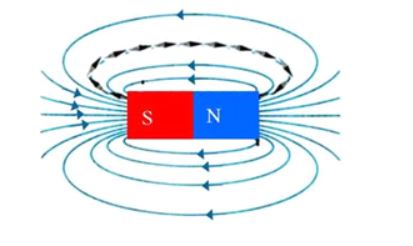
\includegraphics[scale=0.9]{../figs//VN11-2021-PH-TP023-01.JPG}
			\end{center}


	}
	\item \mkstar{1}

	\cauhoi{
		
	Phát biểu nào sau đây là \textbf{không đúng}?
	
	Từ trường đều là từ trường có
	\begin{mcq}
		\item các đường sức song song và cách đều nhau.
		\item cảm ứng từ tại mọi nơi đều bằng nhau.
		\item lực từ tác dụng lên các dòng điện như nhau.
		\item các đặc điểm bao gồm cả phương án A và B.
	\end{mcq}
	}

	\loigiai{
		
	\textbf{Đáp án: C.}
	
	Từ trường đều là từ trường có các đường sức song song và cách đều nhau, cảm ứng từ tại mọi nơi đều bằng nhau.
	
	Suy ra: A, B, D - đúng

	}
	\item \mkstar{1}

	\cauhoi{
		
	Phát biểu nào sau đây là \textbf{đúng}? 
	\begin{mcq}
		\item  Các đường mạt sắt của từ phổ chính là các đường sức từ.
		\item Các đường sức từ của từ trường đều có thể là những đường cong cách đều nhau.
		\item Các đường sức từ là những đường cong kín.
		\item Một hạt mang điện chuyển động theo quỹ đạo tròn trong từ trường thì quỹ đạo chuyển động của hạt chính là một đường sức từ.
	\end{mcq}
	}

	\loigiai{
		
	\textbf{Đáp án: C.}

	}
\end{enumerate}
\section{Lực từ. Cảm ứng từ}
\begin{enumerate}[label=\bfseries Câu \arabic*:]
	
	\item \mkstar{1}
	
	\cauhoi{
		Một dòng điện đặt trong từ trường vuông góc với đường sức từ, chiều của lực từ tác dụng vào dòng điện sẽ không thay đổi khi
		\begin{mcq}
			\item đổi chiều dòng điện ngược lại.
			\item đổi chiều cảm ứng từ ngược lại.
			\item đồng thời đổi chiều dòng điện và đổi chiều cảm ứng từ.
			\item quay dòng điện một góc $90^\circ$ xung quanh đường sức từ.
		\end{mcq}
	}
	
	\loigiai{
		
		\textbf{Đáp án: C.}
		
		Một dòng điện đặt trong từ trường vuông góc với đường sức từ, chiều của lực từ tác dụng vào dòng điện sẽ không thay đổi khi đồng thời đổi chiều dòng điện và đổi chiều cảm ứng từ.
		
	}
	
	\item \mkstar{1}
	
	\cauhoi{
		Phát biểu nào sau đây là \textbf{không đúng}?
		\begin{mcq}
			\item Lực từ tác dụng lên dòng điện có phương vuông góc với dòng điện.
			\item Lực từ tác dụng lên dòng điện có phương vuông góc với đường cảm ứng từ.
			\item Lực từ tác dụng lên dòng điện có phương vuông góc với mặt phẳng chứa dòng điện và đường cảm ứng từ.
			\item Lực từ tác dụng lên dòng điện có phương tiếp tuyến với các đường cảm ứng từ.
		\end{mcq}
	}
	\loigiai{
		
		\textbf{Đáp án: D.}
		
		Ta có:
		
		Lực từ có phương vuông góc với mặt phẳng
		
		Lực từ có phương vuông góc với đường cảm ứng từ và có phương vuông góc với dòng điện
		
		Phương án D - sai
	}
		\item \mkstar{1}
	
	\cauhoi{
		Phát biểu nào sau đây là \textbf{không đúng}?	
		\begin{mcq}
			\item Lực từ tác dụng lên dòng điện đổi chiều khi đổi chiều dòng điện.
			\item Lực từ tác dụng lên dòng điện đổi chiều khi đổi chiều đường cảm ứng từ.
			\item Lực từ tác dụng lên dòng điện đổi chiều khi tăng cường độ dòng điện.
			\item Lực từ tác dụng lên dòng điện không đổi chiều khi đồng thời đổi chiều dòng điện và đường cảm ứng từ.
		\end{mcq}
		
	}
	\loigiai{
		
		\textbf{Đáp án: C.}
		
		Chiều của lực từ không phụ thuộc vào độ lớn của cường độ dòng điện.
	}
		\item \mkstar{1}
	
	\cauhoi{
	Phát biểu nào sau đây là \textbf{không đúng}?
	\begin{mcq}
		\item Lực từ tác dụng lên một đoạn dây dẫn mang dòng điện đặt trong từ trường đều tỉ lệ thuận với cường độ dòng điện trong đoạn dây.
		\item Lực từ tác dụng lên một đoạn dây dẫn mang dòng điện đặt trong từ trường đều tỉ lệ thuận với chiều dài của đoạn dây.
		\item  Lực từ tác dụng lên một đoạn dây dẫn mang dòng điện đặt trong từ trường đều tỉ lệ thuận với góc hợp bởi đoạn dây và đường sức từ.	
		\item Lực từ tác dụng lên một đoạn dây dẫn mang dòng điện đặt trong từ trường đều tỉ lệ thuận với cảm ứng từ tại điểm đặt đoạn dây.
	\end{mcq}
	}
	\loigiai{
		
		\textbf{Đáp án: C.}
		
		 Lực từ tác dụng lên đoạn dây dẫn mang dòng điện được xác định theo công thức $F = BIl \sin \alpha.$
	}
		\item \mkstar{1}
	
	\cauhoi{
		Phát biểu nào dưới đây là đúng?
		
		Cho một đoạn dây dẫn mang dòng điện $I$ đặt song song với đường sức từ, chiều của dòng điện ngược chiều với chiều của đường sức từ. 
		\begin{mcq}
			\item Lực từ luôn bằng không khi tăng cường độ dòng điện
			\item Lực từ tăng khi tăng cường độ dòng điện.	
			\item Lực từ giảm khi tăng cường độ dòng điện.	
			\item Lực từ đổi chiều khi ta đổi chiều dòng điện.
		\end{mcq}
	}
	\loigiai{
		
		\textbf{Đáp án: A.}
		
		 Áp dụng công thức $F = BIl\sin \alpha$ ta thấy khi dây dẫn song song với các đường cảm ứng từ thì $\alpha = 0$, nên khi tăng cường độ dòng điện thì lực từ vẫn bằng không.
	}
	
		\item \mkstar{1}
	
	\cauhoi{
		Phát biểu nào sau đây là \textbf{không đúng}?
		
		Một đoạn dây dẫn thẳng mang dòng điện I đặt trong từ trường đều thì 
		
		\begin{mcq}
			\item lực từ tác dụng lên mọi phần của đoạn dây.
			\item lực từ chỉ tác dụng vào trung điểm của đoạn dây.
			\item lực từ chỉ tác dụng lên đoạn dây khi nó không song song với đường sức từ.
			\item lực từ tác dụng lên đoạn dây có điểm đặt là trung điểm của đoạn dây.
		\end{mcq}
	}
	\loigiai{
		
		\textbf{Đáp án: B.}
		
		Một đoạn dây dẫn thẳng mang dòng điện I đặt trong từ trường đều thì lực từ tác dụng lên mọi phần của đoạn dây.
	}

		\item \mkstar{1}
	
	\cauhoi{
		Phát biểu nào sau đây là \textbf{không đúng}? 
		
		\begin{mcq}
			\item Cảm ứng từ là đại lượng đặc trưng cho từ trường về mặt tác dụng lực. 
			\item Độ lớn của cảm ứng từ được xác định theo công thức $B=\dfrac{F}{Il\sin \alpha}$ phụ thuộc vào cường độ dòng điện $I$ và chiều dài đoạn dây dẫn đặt trong từ trường.
			\item Độ lớn của cảm ứng từ được xác định theo công thức  $B=\dfrac{F}{Il\sin \alpha}$ không phụ thuộc vào cường độ dòng điện $I$ và chiều đài đoạn dây dẫn đặt trong từ trường.
			\item Cảm ứng từ là đại lượng vectơ.
		\end{mcq}
	}
	\loigiai{
		
		\textbf{Đáp án: B}
		
		Cảm ứng từ đặc trưng cho từ trường tại một điểm về phương diện tác dụng lực, phụ thuộc vào bản thân từ trường tại điểm đó.
		
		
	}

		\item \mkstar{1}
	
	\cauhoi{
		Chiều của lực từ tác dụng lên đoạn dây dẫn mang dòng điện, thường được xác định bằng quy tắc
		\begin{mcq}(2)
			\item bàn tay trái.
			\item bàn tay phải.
			\item nắm tay trái.
			\item nắm tay phải.
		\end{mcq}
	}
	\loigiai{
		
		\textbf{Đáp án: A.}
		
		Chiều của lực từ tác dụng lên đoạn dây dẫn mang dòng điện đặt trong trừ trường được xác định bằng quy tắc bàn tay trái.
	}
		\item \mkstar{2}
	
	\cauhoi{
		Một đoạn dây dẫn dài 5 cm đặt trong từ trường đều và vuông góc với vectơ cảm ứng từ. Dòng điện chạy qua dây có cường độ $\text{0,75}$ A. Lực từ tác dụng lên đoạn dây đó là $3\cdot 10^{-2}$ N. Cảm ứng từ của từ trường đó có độ lớn là
		\begin{mcq}(4)
			\item $\text{0,4}\ \text{T}$.
			\item $\text{0,8}\ \text{T}$.
			\item $\text{1,0}\ \text{T}$.	
			\item $\text{1,2}\ \text{T}$.
		\end{mcq}
	}
	\loigiai{
		
		\textbf{Đáp án: B.}
		
		Độ lớn cảm ứng từ
		
		$$B = \dfrac{F}{I l \sin \alpha} = \SI{0,8}{T}.$$
		
		
	}
		\item \mkstar{2}
	
	\cauhoi{
		Một đoạn dây dẫn thẳng MN dài 6 cm có dòng điện I = 5 A đặt trong từ trường đều có cảm ứng từ $B = \text{0,5}\ \text{T}$. Lực từ tác dụng lên đoạn dây có độ lớn $F = \text{7,5}\cdot 10^{-2}\ \text{N}$. Góc $\alpha$ hợp bởi dây MN và đường cảm ứng từ là
		
		\begin{mcq}(4)
			\item $30^\circ$.
			\item $60^\circ$.
			\item $45^\circ$.
			\item $90^\circ$.
		\end{mcq}
	}
	\loigiai{
		
		\textbf{Đáp án: A.}
		
		Góc $\alpha$ hợp bởi dây MN và đường cảm ứng từ là
		
		$$ \sin \alpha = \dfrac{F}{B I l} \Rightarrow \alpha  = 30^\circ.$$
	}
	
	
\end{enumerate}

\section{Từ trường của dòng điện trong các dây dẫn có hình dạng đặc biệt}

\begin{enumerate}[label=\bfseries Câu \arabic*:]
	
		\item \mkstar{1}
	
	\cauhoi{
		
		Cảm ứng từ bên trong một ống dây điện hình trụ, có độ lớn tăng lên khi
		\begin{mcq}
			\item chiều dài hình trụ tăng lên.
			\item đường kính hình trụ giảm đi.
			\item số vòng dây quấn trên một đơn vị chiều dài tăng lên.
			\item cường độ dòng điện giảm đi.
		\end{mcq}
	}
	\loigiai{
		
		\textbf{Đáp án: C.}
		
		Cảm ứng từ bên trong ống dây hình trụ là $B = 4\pi \cdot 10^{-7} nI \Rightarrow B$ tăng khi $n$ tăng.
	}
	
		\item \mkstar{1}
	
	\cauhoi{
		
		Một dây dẫn có dòng điện chạy qua uốn thành vòng tròn. Tại tâm vòng tròn, cảm ứng từ sẽ giảm khi
		\begin{mcq}
			\item cường độ dòng điện tăng lên.
			\item cường độ dòng điện giảm đi.
			\item số vòng dây cuốn sít nhau, đồng tâm tăng lên.
			\item đường kính vòng dây giảm đi.
		\end{mcq}
	}
	\loigiai{
		
		\textbf{Đáp án: B.}
		
		Cảm ứng từ tại tâm vòng tròn là $B = 2 \pi \dot 10^{-7} \dfrac{I}{R} \Rightarrow $   $B$ giảm khi $I$ giảm.
		
	 
		
	
	}
		\item \mkstar{2}
	
	\cauhoi{
		
		Một khung dây dẫn tròn mỏng phẳng gồm 500 vòng dây, bán kính của mỗi vòng dây là 10 cm, đặt trong chân không. Dòng điện chạy trong các vòng dây có cường độ $I = \SI{10}{A}$. Cảm ứng từ tại tâm O của khung dây có độ lớn gần đúng là
		\begin{mcq}(4)
			\item $\SI{0,031}{T}$.
			\item $\SI{0,042}{T}$.
			\item $\SI{0,051}{T}$.
			\item $\SI{0,022}{T}$.
		\end{mcq}
	}
	\loigiai{
		
		\textbf{Đáp án: A.}
		
		Cảm ứng từ tại tâm O của khung dây có độ lớn gần đúng là:
		
		$$B = 2 \pi \dot 10^{-7} \dfrac{NI}{R}  =  \SI{0,031}{T}$$ 
	}
		\item \mkstar{2}
	
	\cauhoi{
		
		Một ống dây hình trụ, tiết diện đều, không có lõi thép. Số vòng dây trên mỗi mét chiều dài ống là 5000 vòng. Nếu cường độ dòng điện chạy trên mỗi vòng của ống dây là 12 A thì cảm ứng từ trong lòng của ống dây có độ lớn bằng
		\begin{mcq}(4)
			\item $\text{75,4}\ \mu \text{T}$.
			\item $\SI{754}{mT}$.
			\item $\SI{75,4}{mT}$.
			\item $\SI{0,754}{T}$.
		\end{mcq}
	}
	\loigiai{
		
		\textbf{Đáp án: C.}
		
		Cảm ứng từ trong lòng của ống dây có độ lớn bằng:
		
		$$B = 4 \pi \cdot 10^{-7}nI = 754 \cdot 10^{-4}\ \text T.$$
		
		
	}
			\item \mkstar{2}
		
		\cauhoi{
			Nếu cường độ dòng điện trong dây dẫn tròn tăng 2 lần và đường kính dòng điện tăng 2 lần thì cảm ứng từ tại tâm vòng dây
			
			\begin{mcq}(4)
				\item không đổi.
				\item tăng 2 lần.
				\item tăng 4 lần.
				\item giảm 2 lần.
			\end{mcq}
		}
		\loigiai{
			
			\textbf{Đáp án: A.}
			
			Ta có:
			
			$$B = 2 \pi \dot 10^{-7} \dfrac{I}{R}.$$
			
			Nếu $I$ tăng 2 và $R$ tăng 2 thì $B$ không đổi.
		}
	
	
\end{enumerate}

\section{Lực Lo-ren-xơ}
\begin{enumerate}[label=\bfseries Câu \arabic*:]
	
	\item \mkstar{1} 
	
	\cauhoi{
		Trong hình vẽ sau hình nào chỉ đúng hướng của lực Lorenxơ tác dụng lên hạt mang điện dương chuyển động trong từ trường đều?
		\begin{mcq}(2)
			\item 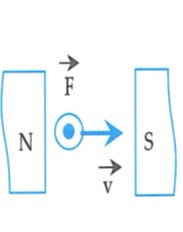
\includegraphics[scale=0.8]{../figs/VN11-PH-27-P-018-1-h1.jpg}
			\item 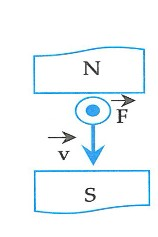
\includegraphics[scale=0.8]{../figs/VN11-PH-27-P-018-1-h2.jpg}
			\item 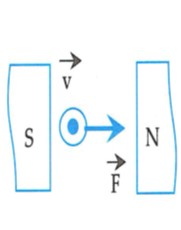
\includegraphics[scale=0.8]{../figs/VN11-PH-27-P-018-1-h3.jpg}
			\item 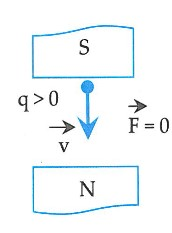
\includegraphics[scale=0.8]{../figs/VN11-PH-27-P-018-1-h4.jpg}
		\end{mcq}
	}
	
	\loigiai{
		\textbf{Đáp án: D.}
		
	
	}
	
	\item \mkstar{1} 
	
	\cauhoi{
		Trong hình vẽ sau hình nào chỉ đúng hướng của lực Lorenxơ tác dụng lên electron chuyển động trong từ trường đều?
		\begin{mcq}(2)
			\item 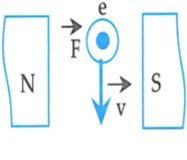
\includegraphics[scale=0.8]{../figs/VN11-PH-27-P-018-1-h5.jpg}
			\item 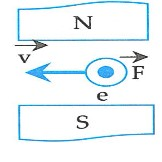
\includegraphics[scale=0.8]{../figs/VN11-PH-27-P-018-1-h6.jpg}
			\item 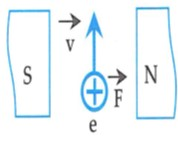
\includegraphics[scale=0.8]{../figs/VN11-PH-27-P-018-1-h7.jpg}
			\item 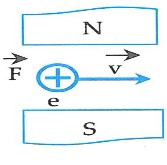
\includegraphics[scale=0.8]{../figs/VN11-PH-27-P-018-1-h8.jpg}
		\end{mcq}
		
	}
	\loigiai{
		
		\textbf{Đáp án: C}
	}
	
	\item \mkstar{1}
	
	\cauhoi{
		Trong hình vẽ sau hình nào chỉ đúng hướng của lực Lorenxơ tác dụng lên electron và hạt mang điện dương chuyển động trong từ trường đều?
		\begin{mcq} (2)
			\item 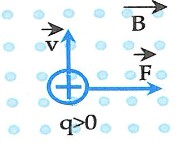
\includegraphics[scale=0.8]{../figs/VN11-PH-27-P-018-1-h9.jpg}
			\item 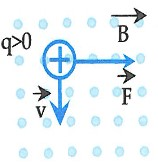
\includegraphics[scale=0.8]{../figs/VN11-PH-27-P-018-1-h10.jpg}
			\item 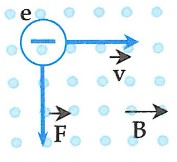
\includegraphics[scale=0.8]{../figs/VN11-PH-27-P-018-1-h11.jpg}
			\item 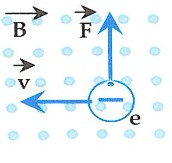
\includegraphics[scale=0.8]{../figs/VN11-PH-27-P-018-1-h12.jpg}
		\end{mcq}
		
	}
	\loigiai{
		
	\textbf{Đáp án: A.}
	}
	\item \mkstar{1}
	
	\cauhoi{
		Trong hình vẽ sau hình nào chỉ đúng hướng của lực Lorenxơ tác dụng lên electron chuyển động trong từ trường đều?
		\begin{mcq}(2)
			\item 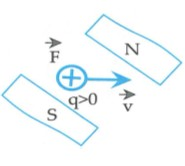
\includegraphics[scale=0.8]{../figs/VN11-PH-27-P-018-1-h13.jpg}
			\item 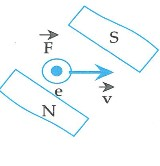
\includegraphics[scale=0.8]{../figs/VN11-PH-27-P-018-1-h14.jpg}
			\item 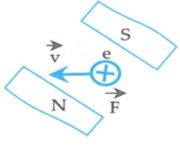
\includegraphics[scale=0.8]{../figs/VN11-PH-27-P-018-1-h15.jpg}
			\item 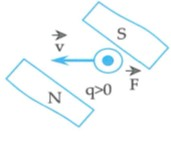
\includegraphics[scale=0.8]{../figs/VN11-PH-27-P-018-1-h16.jpg}
		\end{mcq}
		
	}
	\loigiai{
		
		\textbf{Đáp án: A}
	}
\end{enumerate}	
\whiteBGstarEnd